\documentclass[11pt,a4paper]{myclass}
\usepackage{tkz-tab}
\SetWatermarkText{\expandafter\mlfamily រៀបរៀងដោយ វិទ្យាស្ថានបច្ចេកវិទ្យាកម្ពុជា}
\begin{document}
	\begin{minipage}[t]{.425\linewidth}
		\mlfamily\openup=2pt
		ប្រឡងសាកល្បងមធ្យមសិក្សាទុតិយភូមិ\\
		សម័យប្រឡង ៖ \dotfill\\
		វិញ្ញាសា​ ៖ គណិតវិទ្យា (ថ្នាក់វិទ្យាសាស្ត្រ)\\
		រយៈពេល ៖ ១៥០ នាទី\\
		ពិន្ទុ ៖ ១២៥
	\end{minipage}~\hfill~
	\begin{minipage}[t]{.425\linewidth}
		\mlfamily\openup=2pt
		មណ្ឌលប្រឡង ៖ \dotfill\\
		លេខតុ ៖ \dotfill\ លេខបន្ទប់ ៖ \dotfill\\
		ឈ្មោះបេក្ខជន ៖ \dotfill\\
		ហត្ថលេខាបេក្ខជន ៖ \dotfill\\
		\hphantom{ក}
	\end{minipage}
	\vskip-\baselineskip
	\centerline{\mlfamily ប្រធាន}
	\begin{enumerate}
		\item គេមានចំនួនកុំផ្លិច $ z_1=\frac{\sqrt{3}}{2}+i\frac{1}{2} $ និង $ z_2=-1+i\sqrt{3} $~។
		\begin{enumerate}
			\item បង្ហាញថា $ z_2=2iz_1 $~។
			\item សរសេរ $ z_1 $ និង $ z_2 $ ជាទម្រង់ត្រីកោណមាត្រ។
			\item បង្ហាញថា $ \left(\cos\frac{\pi}{6}-i\sin\frac{\pi}{6}\right)z_1=1 $ រួចសរសេរ $ \frac{1}{(z_1)^4} $ ជាទម្រង់ពីជគណិត~។
		\end{enumerate}
		\item គណនាលីមីត
		\begin{Enumerate}(3)
			\item $ \lim\limits_{x\to 1}\frac{x^3-3x+2}{x^2-1} $
			\item $ \lim\limits_{x\to 0}\frac{x^2-\sin 3x}{2x} $
			\item $ \lim\limits_{x\to 2}\frac{x\sqrt{2+x}-4}{8-x^3} $
		\end{Enumerate}
		\item គេមានអនុគមន៍ $ f(x)=\frac{2x+3}{x^2-6x+9} $ កំណត់ចំពោះគ្រប់ $ x\neq 3 $~។
		\begin{enumerate}
			\item កំណត់ចំនួនពិត $ A $ និង $ B $ ដែល $ f(x)=\frac{A}{x-3}+\frac{B}{(x-3)^2} $~។
			\item គណនាអាំងតេក្រាលកំណត់ $ I=\int_{1}^{2}\frac{2x+3}{x^2-6x+9}dx $~។
		\end{enumerate}
		%
		\item នៅក្នុងកន្ត្រកមួយមានពងទា``កូន''ចំនួន $ 5 $ គ្រាប់ ពងទា``សាប''ចំនួន $ 7 $ គ្រាប់ និងពងទា``ខូច''ចំនួន $ 3 $ គ្រាប់។ ក្មេងម្នាក់ចាប់យកពងទា $ 5 $ គ្រាប់ ដោយចៃដន្យពីក្នុងកន្ត្រកនោះ។
		គណនាប្រូបាបនៃព្រឹត្តិការណ៍៖
		\begin{enumerate}
			\item $ A: $ ``ចាប់បានពងទាកូន $ 2 $ គ្រាប់ ពងទាសាប $ 2 $ គ្រាប់ និងពងទាខូច $ 1 $ គ្រាប់''~។
			\item $ B: $ ``ចាប់បានពងទាកូន $ 4 $ គ្រាប់''~។
			\item $ C: $ ``ចាប់បានពងទាខូចយ៉ាងតិច $ 1 $ គ្រាប់''~។
		\end{enumerate}
		%
		\item តាង $ (C) $ ជាខ្សែកោងតាងអនុគមន៍ $ y=f(x) $ ដែលផ្ទៀងផ្ទាត់ $ y''+3y'-18y=0 $~។ កំណត់អនុគន៍ $ y=f(x) $ បើដឹងថា $ (C) $ កាត់តាមគល់ $ O $ និងមានសមីការបន្ទាត់ប៉ះត្រង់ $ O $ គឺ $ y=-9x $~។
		%
		\item អនុគមន៍ $ f $ កំណត់ចំពោះគ្រប់តម្លៃចំនួនពិត $ x $ ដោយ
		$ f(x)=x-2+\dfrac{8}{e^x+2} $ ដែលក្រាបវាតាងដោយ $ C $~។
		\begin{enumerate}
			\item គណនាលីមីតនៃអនុគមន៍ $ f $ ត្រង់ $ -\infty $ និង $ +\infty $~។
			\item បង្ហាញថាបន្ទាត់ $ L_1:\;y=x-2 $ និង $ L_2:\;y=x+2 $ ជាអាស៊ីមតូតទ្រេតនៃក្រាប $ C $ ខាងមែក $ +\infty $ និង $ -\infty $ រៀងគ្នា។
			\item សិក្សាទីតាំងក្រាប $ C $ ធៀបនឹងបន្ទាត់ $ L_1 $ រួចធៀបនឹងបន្ទាត់ $ L_2 $~។
			\item បង្ហាញថាដេរីវេ $ f'(x)=\left(\dfrac{e^x-2}{e^x+2}\right)^2 $ និងសរសេរសមីការបន្ទាត់ $ T $ ប៉ះក្រាប $ C $ ត្រង់ចំណុចដែលមានអាប់ស៊ីស $ \ln 2 $~។
			\item សង់តារាងអថេរភាពនៃអនុគមន៍ $ f $~។
			\item សង់ក្រាប $ C $ បន្ទាត់ $ T $ និងអាស៊ីមតូត $ L_1,L_2 $ ក្នុងតម្រុយតែមួយ។\\
			គេយក $ e^{-1}=0.4,e=2.7,e^2=7.4 $ និង $ \ln 2=0.7 $~។
		\end{enumerate}
		%
		\item ក្នុងលំហរប្រដាប់ដោយតម្រុយអរតូណរម៉ាល់ $ (O;\vec{i},\vec{j},\vec{k}) $ គេឲ្យបួនចំណុច $ A(3,3,4),\,B(1,3,4),\,C(1,-1,2) $ និង $ D(3,-1,2) $~។%translation of A(1,2,1),B(-1,2,1),C(-1,-2,-1),D(1,-2,-1) by u=(2,1,3)
		\begin{enumerate}
			\item ចូរសរសេរវ៉ិចទ័រ $ \overrightarrow{AB},\,\overrightarrow{DC},\,\overrightarrow{AD},\,\overrightarrow{BC} $~។
			\item គណនាផលគុណស្កាលែ $ \overrightarrow{AB}\cdot\overrightarrow{AD} $ រួចប្រាប់ប្រភេទចតុកោណ $ ABCD $~។
			\item គណនាប្រវែង $ AB $ និង $ AD $ រួចផ្ទៃក្រឡាត្រីកោណ $ \Delta ABD $~។
			\item គណនាផលគុណវ៉ិចទ័រ $ \overrightarrow{AB}\times \overrightarrow{AD} $ និងសរសេរវ៉ិចទ័រ $ \overrightarrow{AO} $~។
			\item គណនាមាឌចតុមុខ $ OABD $ ដែល $ O(0,0,0) $ ជាគល់តម្រុយកូអរដោនេ រួចគណនាចម្ងាយពី $ O $ ទៅប្លង់ $ (ABD) $។
		\end{enumerate}
		%
	\end{enumerate}
	\newpage
	\centerline{\expandafter\mlfamily ចម្លើយ}
	\begin{enumerate}
		\item គេមានចំនួនកុំផ្លិច $ z_1=\frac{\sqrt{3}}{2}+i\frac{1}{2} $ និង $ z_2=-1+i\sqrt{3} $
		\begin{enumerate}
			\item បង្ហាញថា $ z_2=2iz_1 $
			\begin{align*}
			z_2=i^2+i\sqrt{3}=2i\left( \frac{1}{2}i+\frac{\sqrt{3}}{2} \right)=2iz_1
			\end{align*}
			\item សរសេរ $ z_1 $ និង $ z_2 $ ជាទម្រង់ត្រីកោណមាត្រ
			\begin{align*}
			z_1 &=\frac{\sqrt{3}}{2}+i\frac{1}{2}=\cos \frac{\pi}{6}+i\sin\frac{\pi}{6}\\
			z_2 &=-1+i\sqrt{3}=2\left( -\frac{1}{2}+i\frac{\sqrt{3}}{2} \right)\\
			&=2\left[\cos\left( \pi-\frac{\pi}{6} \right)+i\sin\left( \pi-\frac{\pi}{6} \right) \right]\\
			&=2\left( \cos \frac{5\pi}{6}+i\sin\frac{5\pi}{6} \right)
			\end{align*}
			\item បង្ហាញថា $ \left(\cos\frac{\pi}{6}-i\sin\frac{\pi}{6}\right)z_1=1 $ រួចសរសេរ $ \frac{1}{(z_1)^4} $ ជាទម្រង់ពីជគណិត
			\begin{align*}
			\left( \cos\frac{\pi}{6}-i\sin\frac{\pi}{6} \right)z_1
			&=\left( \cos\frac{\pi}{6}-i\sin\frac{\pi}{6} \right)\left( \cos\frac{\pi}{6}+i\sin\frac{\pi}{6} \right)\\
			&=\cos^2\frac{\pi}{6}+\sin^2\frac{\pi}{6}=1\\
			\Rightarrow
			\frac{1}{(z_1)^4} &=\left( \cos\frac{\pi}{6}-i\sin\frac{\pi}{6} \right)^4\\
			&=\left[ \cos\left( -\frac{\pi}{6} \right)+i\sin\left( -\frac{\pi}{6} \right) \right]^4\\
			&=\cos\left[ 4\left( -\frac{\pi}{6} \right) \right]+i\sin\left[ 4\left( -\frac{\pi}{6} \right) \right]\\
			&=\cos\left( -\frac{2\pi}{3} \right)+i\sin\left( -\frac{2\pi}{3} \right)\\
			&=\cos\frac{2\pi}{3}-i\sin\frac{2\pi}{3}\\
			&=\cos\left( \pi-\frac{\pi}{3} \right)-i\sin\left( \pi-\frac{\pi}{3} \right)\\
			&=-\cos\frac{\pi}{3}-i\sin\frac{\pi}{3}\\
			&=-\frac{1}{2}-i\frac{\sqrt{3}}{2}
			\end{align*}
		\end{enumerate}
		\item គណនាលីមីត
		\begin{enumerate}[k]
			\item $ \lim\limits_{x\to 1}\frac{x^3-3x+2}{x^2-1} $ រាងមិនកំណត់ $ \frac{0}{0} $
			\begin{align*}
			\lim\limits_{x\to 1}\frac{x^3-3x+2}{x^2-1} 
			&=\lim\limits_{x\to 1}\frac{x^3-x-2x+2}{x^2-1}\\
			&=\lim\limits_{x\to 1}\left( x-\frac{2(x-1)}{(x-1)(x+1)} \right)\\
			&=\lim\limits_{x\to 1}\left( x-\frac{2}{x+1} \right)\\
			&=1-1=0
			\end{align*}
			\item $ \lim\limits_{x\to 0}\frac{x^2-\sin 3x}{2x} $ រាងមិនកំណត់ $ \frac{0}{0} $
			\begin{align*}
			\lim\limits_{x\to 0}\frac{x^2-\sin 3x}{2x}
			&=\lim\limits_{x\to 0}\left( \frac{x}{2}-\frac{\sin 3x}{2x} \right)\\
			&=\lim\limits_{x\to 0}\left( \frac{x}{2}-\frac{\sin 3x}{3x}\times\frac{3}{2} \right)\\
			&=\frac{x}{2}-\frac{3}{2}=-\frac{3}{2}
			\end{align*}
			\item $ \lim\limits_{x\to 2}\frac{x\sqrt{2+x}-4}{8-x^3} $ រាងមិនកំណត់ $ \frac{0}{0} $
			\begin{align*}
			\lim\limits_{x\to 2}\frac{x\sqrt{2+x}-4}{8-x^3}
			&=\lim\limits_{x\to 2}\frac{x^2(2+x)-16}{-(x^3-8)(x\sqrt{2+x}+4)}\\
			&=\lim\limits_{x\to 2}\frac{x^3+2x^2-16}{-(x-2)(x^2+2x+4)(x\sqrt{2+x}+4)}\\
			&=\lim\limits_{x\to 2}\frac{x^3-2x^2+4x^2-16}{-(x-2)(x^2+2x+4)(x\sqrt{2+x}+4)}\\
			&=\lim\limits_{x\to 2}\frac{(x-2)(x^2+4(x+2))}{-(x-2)(x^2+2x+4)(x\sqrt{2+x}+4)}\\
			&=\lim\limits_{x\to 2}\frac{x^2+4(x+2)}{-(x^2+2x+4)(x\sqrt{2+x}+4)}\\
			&=\frac{4+16}{-12\times 8}=-\frac{5}{24}
			\end{align*}
		\end{enumerate}
		\item គេមានអនុគមន៍ $ f(x)=\frac{2x+3}{x^2-6x+9} $ កំណត់ចំពោះគ្រប់ $ x\neq 3 $
		\begin{enumerate}
			\item កំណត់ចំនួនពិត $ A $ និង $ B $ ដែល $ f(x)=\frac{A}{x-3}+\frac{B}{(x-3)^2} $
			\begin{align*}
			f(x) &=\frac{A(x-3)+B}{(x-3)^2}
			\end{align*}
			នោះគេបាន
			\begin{align*}
			A(x-3)+B &=2x+3\quad\text{គ្រប់}\; x\in\mathbb{R}
			\end{align*}
			\begin{itemize}
				\item យក $ x=3 $ គេបាន $ B=9 $
				\item យក $ x=4 $ គេបាន $ A+9=11 $ នាំឲ្យ $ A=3 $
			\end{itemize}
			ដូច្នេះ $ A=3,B=9 $~។
			\item គណនាអាំងតេក្រាលកំណត់ $ I=\int_{1}^{2}\frac{2x+3}{x^2-6x+9}dx $
			\begin{align*}
			I &=\int_{1}^{2}\frac{2x+3}{x^2-6x+9}dx\\
			&=\int_{1}^{2}\left( \frac{3}{x-3}+\frac{9}{(x-3)^2} \right)dx\\
			&=\left.\left( 3\ln|x-3|-\frac{9}{x-3} \right)\right|_{1}^{2}\\
			&=\frac{9}{2}-\ln (4)
			\end{align*}
		\end{enumerate}
		%
		\item នៅក្នុងកន្ត្រកមួយមានពងទា``កូន''ចំនួន $ 5 $ គ្រាប់ ពងទា``សាប''ចំនួន $ 7 $ គ្រាប់ និងពងទា``ខូច''ចំនួន $ 3 $ គ្រាប់។ ក្មេងម្នាក់ចាប់យកពងទា $ 5 $ គ្រាប់ ដោយចៃដន្យពីក្នុងកន្ត្រកនោះ។
		គណនាប្រូបាបនៃព្រឹត្តិការណ៍៖\\
		ចំនួនករណីអាច $ n(S)=C(15,5)=\frac{15\cdot 14\cdot 13\cdot 12\cdot 11}{1\cdot 2\cdot 3\cdot 4\cdot 5}=3003 $
		\begin{enumerate}
			\item $ A: $ ``ចាប់បានពងទាកូន $ 2 $ គ្រាប់ ពងទាសាប $ 2 $ គ្រាប់ និងពងទាខូច $ 1 $ គ្រាប់''
			\begin{align*}
			P(B) &=\frac{n(A)}{n(S)}
			=\frac{C(5,2)C(7,2)C(3,1)}{3003}
			=\frac{10\cdot 21\cdot 3}{3003}
			=\frac{30}{143}
			\end{align*}
			\item $ B: $ ``ចាប់បានពងទាកូន $ 4 $ គ្រាប់''
			\begin{align*}
			P(B) &=\frac{n(A)}{n(S)}
			=\frac{C(5,4)C(10,1)}{3003}
			=\frac{50}{3003}
			\end{align*}
			\item $ C: $ ``ចាប់បានពងទាខូចយ៉ាងតិច $ 1 $ គ្រាប់''\\
			$ \overline{C}: $ ``ចាប់បានពងទាខូចយ៉ាងតិច $ 1 $ គ្រាប់''
			\begin{align*}
			P(C)=1-P(\overline{C})=1-\frac{C(10,5)}{3003}
			=\frac{12}{143}
			\end{align*}
		\end{enumerate}
		%
		\item តាង $ (C) $ ជាខ្សែកោងតាងអនុគមន៍ $ y=f(x) $ ដែលផ្ទៀងផ្ទាត់ $ y''+3y'-18y=0 $~។ កំណត់អនុគន៍ $ y=f(x) $ បើដឹងថា $ (C) $ កាត់តាមគល់ $ O $ និងមានសមីការបន្ទាត់ប៉ះត្រង់ $ O $ គឺ $ y=-9x $~។\\
		%
		សមីការសម្គាល់
		\begin{align*}
		r^2+3r-18 &=0\\
		(r-3)(r+6) &=0\\
		r_1=3,r_2&=-6
		\end{align*}
		នោះសមីការឌីផេរ៉ង់ស្យែលមានចម្លើយ $ y=Ae^{3x}+Be^{-6x} $~។ តាមសម្មតិកម្ម $ y(0)=0 $ និង $ y'(0)=-9 $ នោះ
		\begin{align*}
		\begin{cases}
		A+B=0\\
		3A-6B=-9
		\end{cases}
		\Rightarrow
		\begin{cases}
		A=-1\\
		B=1
		\end{cases}
		\end{align*}
		សមីការឌីផេរ៉ង់ស្យែលមានចម្លើយ $ y=-e^{3x}+e^{-6x} $~។
		\item អនុគមន៍ $ f $ កំណត់ចំពោះគ្រប់តម្លៃចំនួនពិត $ x $ ដោយ
		$ f(x)=x-2+\dfrac{8}{e^x+2} $ ដែលក្រាបវាតាងដោយ $ C $~។
		\begin{enumerate}
			\item គណនាលីមីតនៃអនុគមន៍ $ f $ ត្រង់ $ -\infty $ និង $ +\infty $
			\begin{align*}
			\lim\limits_{x\to -\infty}f(x)
			&=\lim\limits_{x\to -\infty} \left( x-2+\frac{8}{e^2+2} \right)=-\infty\\
			\lim\limits_{x\to +\infty}f(x)
			&=\lim\limits_{x\to +\infty} \left( x-2+\frac{8}{e^2+2} \right)=+\infty
			\end{align*}
			\item បង្ហាញថាបន្ទាត់ $ L_1:\;y=x-2 $ និង $ L_2:\;y=x+2 $ ជាអាស៊ីមតូតទ្រេតនៃក្រាប $ C $ ខាងមែក $ +\infty $ និង $ -\infty $ រៀងគ្នា
			\begin{align*}
			\lim\limits_{x\to +\infty}\left[ f(x)-(x-2) \right]
			&=\lim\limits_{x\to +\infty}\frac{8}{e^x+2}=0\\
			\lim\limits_{x\to +\infty}\left[ f(x)-(x+2) \right]
			&=\lim\limits_{x\to +\infty}\frac{-2e^x}{e^x+2}=0
			\end{align*}
			ដូច្នេះ បន្ទាត់ $ L_1:\;y=x-2 $ និង $ L_2:\;y=x+2 $ ជាអាស៊ីមតូតទ្រេតនៃក្រាប $ C $ ខាងមែក $ +\infty $ និង $ -\infty $ រៀងគ្នា។
			\item សិក្សាទីតាំងក្រាប $ C $ ធៀបនឹងបន្ទាត់ $ L_1 $ រួចធៀបនឹងបន្ទាត់ $ L_2 $
			\begin{itemize}
				\item $ f(x)-(x-2)=\frac{8}{e^x+2}>0 $ គ្រប់ $ x\in\mathbb{R} $ នោះខ្សែកោង $ (C) $ នៅលើបន្ទាត់ $ L_1 $ ជានិច្ច។
				\item $ f(x)-(x+2)=-\frac{2e^x}{e^x+2}<0 $ គ្រប់ $ x\in\mathbb{R} $ នោះខ្សែកោង $ (C) $ នៅក្រោមបន្ទាត់ $ (L_2) $ ជានិច្ច។
			\end{itemize}
			\item បង្ហាញថាដេរីវេ $ f'(x)=\left(\dfrac{e^x-2}{e^x+2}\right)^2 $ និងសរសេរសមីការបន្ទាត់ $ T $ ប៉ះក្រាប $ C $ ត្រង់ចំណុចដែលមានអាប់ស៊ីស $ \ln 2 $
			\begin{align*}
			f'(x) &= 1-\frac{8e^x}{(e^x+2)}=\frac{(e^x+2)^2-4e^x}{(e^x+2)^2}=\left( \frac{e^x-2}{e^x+2} \right)^2
			\end{align*}
			សមីការបន្ទាត់ប៉ះ $ (T):y=f'(\ln 2)(x-\ln 2)+f(\ln 2) $ ដោយ
			\begin{align*}
			f'(\ln 2) &=\left( \frac{e^{\ln 2}-2}{e^{\ln 2}+2} \right)^2=0\\
			f(\ln 2) &=\ln 2-2+\frac{8}{e^{\ln 2}+2}=\ln 2
			\end{align*}
			ដូច្នេះ សមីការបន្ទាត់ប៉ះត្រង់ $ x=\ln 2 $ គឺ $ (T):y=\ln 2 $~។
			\item សង់តារាងអថេរភាពនៃអនុគមន៍ $ f $
			\begin{figure}[H]
				\centering
				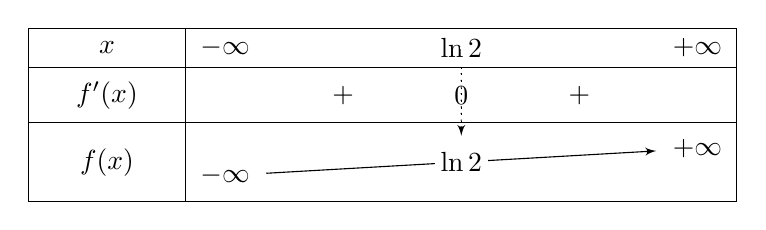
\begin{tikzpicture}
				\tkzTabInit{$ x $/.5,$ f'(x) $/.7,$ f(x) $/1}{$ -\infty $,$ \ln 2 $,$ +\infty $}
				\tkzTabLine{,+,z,+,}
				\tkzTabVar{-/$ -\infty $,R/,+/$ +\infty $}
				\tkzTabVal[draw]{1}{3}{0.5}{}{$ \ln 2 $}
				\end{tikzpicture}
			\end{figure}
			\item សង់ក្រាប $ C $ បន្ទាត់ $ T $ និងអាស៊ីមតូត $ L_1,L_2 $ ក្នុងតម្រុយតែមួយ
			\begin{figure}[H]
				\centering
				\begin{tikzpicture}
				\draw[->](-5,0)node[left]{$x'$}--(5,0)node[right]{$x$};
				\draw[->](0,-5)node[below]{$y'$}--(0,5)node[above]{$y$};
				\draw[line width=1pt] plot[domain=-5:5,samples=50]({\x},{\x-2+8/(exp(\x)+2)});
				\draw(-3,-5)--node[sloped,near start,above]{$ (L_2):y=x+2 $}(5,3);
				\draw(-5,-3)--node[sloped,near start,above]{$ (L_1):y=x+2 $}(3,5);
				\fill({ln(2)},{ln(2)})circle(1.5pt);
				\draw(-5,{ln(2)})--node[sloped,near start,above]{$ (T):y=\ln 2 $}(5,{ln(2)});
				\end{tikzpicture}
			\end{figure}
		\end{enumerate}
		%
		\item ក្នុងលំហរប្រដាប់ដោយតម្រុយអរតូណរម៉ាល់ $ (O;\vec{i},\vec{j},\vec{k}) $ គេឲ្យបួនចំណុច $ A(3,3,4),\,B(1,3,4),\,C(1,-1,2) $ និង $ D(3,-1,2) $~។%translation of A(1,2,1),B(-1,2,1),C(-1,-2,-1),D(1,-2,-1) by u=(2,1,3)
		\begin{enumerate}
			\item ចូរសរសេរវ៉ិចទ័រ $ \overrightarrow{AB},\,\overrightarrow{DC},\,\overrightarrow{AD},\,\overrightarrow{BC} $
			\begin{align*}
			\overrightarrow{AB} &=-2\vec{i}\\
			\overrightarrow{DC} &=-2\vec{i}\\
			\overrightarrow{AD} &=-4\vec{j}-2\vec{k}\\
			\overrightarrow{BC} &=-4\vec{j}-2\vec{k}
			\end{align*}
			\item គណនាផលគុណស្កាលែ $ \overrightarrow{AB}\cdot\overrightarrow{AD} $ រួចប្រាប់ប្រភេទចតុកោណ $ ABCD $
			\begin{align*}
			\overrightarrow{AB}\cdot\overrightarrow{AD}
			&=(-2)(0)+(0)(-4)+(0)(-2)=0
			\end{align*}
			ដោយ $ \overrightarrow{AB}=\overrightarrow{DC} $ និង $ \overrightarrow{AB}\cdot\overrightarrow{AD}=0 $ ដូច្នេះ $ ABCD $ ជាចតុកោណកែង។
			\item គណនាប្រវែង $ AB $ និង $ AD $ រួចផ្ទៃក្រឡាត្រីកោណ $ \Delta ABD $
			\begin{align*}
			AB &=\sqrt{(-2)^2+0^2+0^2}=2\\
			AD &=\sqrt{0^2+(-4)^2+(-2)^2}=2\sqrt{5}
			\end{align*}
			ត្រីកោណ $ ABD $ ជាត្រីកោណកែងត្រង់ $ A $ នោះផ្ទៃក្រឡា $ ABD $ គឺ
			\begin{align*}
			S_{\Delta ABC} &=\frac{1}{2}\times AB\times AD=\frac{1}{2}(2)(2\sqrt{5})=2\sqrt{5}
			\end{align*}
			\item គណនាផលគុណវ៉ិចទ័រ $ \overrightarrow{AB}\times \overrightarrow{AD} $ និងសរសេរវ៉ិចទ័រ $ \overrightarrow{AO} $
			\begin{align*}
			\overrightarrow{AB}\times \overrightarrow{AD}
			&=\begin{vmatrix*}[r]
			\vec{i} & \vec{j} & \vec{k}\\
			-2 & 0 & 0\\
			0 & -4 & -2
			\end{vmatrix*}
			=\begin{vmatrix*}[r]
			0 & 0\\
			-4 & -2
			\end{vmatrix*}\vec{i}
			-\begin{vmatrix*}[r]
			-2& 0\\
			0 & -2
			\end{vmatrix*}\vec{j}
			+\begin{vmatrix*}[r]
			-2 & 0\\
			0 & -4 
			\end{vmatrix*}\vec{k}\\
			&=-4\vec{j}+8\vec{k}\\
			\overrightarrow{AO} &=-3\vec{i}-3\vec{j}-4\vec{k}
			\end{align*}
			\item គណនាមាឌចតុមុខ $ OABD $ ដែល $ O(0,0,0) $ ជាគល់តម្រុយកូអរដោនេ រួចគណនាចម្ងាយពី $ O $ ទៅប្លង់ $ (ABD) $
			\begin{align*}
			V_{OABD} &=\frac{1}{6}\left| (\overrightarrow{AB}\times \overrightarrow{AD})\cdot \overrightarrow{AO} \right|\\
			&=\frac{1}{6}\left| (0)(-3)+(-4)(-3)+(8)(-4) \right|=\frac{10}{3}\\
			V_{OABD} &=\frac{1}{3}\times S_{\Delta ABD}\times d(O,ABD)\\
			\Rightarrow
			d(O,ABD) &=\frac{3V_{OABD}}{S_{\Delta ABD}}
			=\frac{3\left( \frac{10}{3} \right)}{2\sqrt{5}}
			=\sqrt{5}
			\end{align*}
		\end{enumerate}
		%
	\end{enumerate}
\end{document}